\documentclass[letterpaper,11pt]{article}
\usepackage{geometry}
\usepackage{graphicx}
\usepackage{hyperref}
\usepackage{tabularx}
\usepackage{multicol}
\usepackage{enumitem}
\geometry{margin=3cm}

\title{

\includegraphics[width=0.4\linewidth]{usi_logo.png}\\
Universit\`a della Svizzera italiana (USI)
\thanks{Download the logo from https://www.usi.ch/en/node/1245}
}
\author{}
\date{}
%%%%%%%%%%%%%%%%%%%%%%%%%%%%%%%%%%%%%%%%%%%%%%%%%%%%%%%%%%%%%%%%%%%%%%%%%%%%%%%%%%%%%%%%%%%%%%%

\begin{document}

\maketitle

\section*{Abstract}
This document provides a brief introduction of the \textit{Universit\`a della Svizzera italiana (USI)\footnotemark}.
Section \ref{section:1} provides some general information about the university. 
Section \ref{section:2} introduces the USI’s departments, and Section \ref{section:2.4} provides more detailed information about the the Faculty of Informatics.

\footnotetext{Formerly known as \textit{University of Lugano.}}

\tableofcontents
\newpage    

%%%%%%%%%%%%%%%%%%%%%%%%%%%%%%%%%%%%%%%%%%%%%%%%%%%%%%%%%%%%%%%%%%%%%%%%%%%%%%%%%%%%%%%%%%%%%%
\section{Introduction}
\label{section:1}
The \textbf{Universit\`a della Svizzera italiana} (USI, literally University of Italian Switzerland), sometimes referred to as the \textbf{University of Lugano}, in English-speaking contexts, is a public Swiss university established in 1995, with campuses in Lugano (see Figure \ref{figure:1}), Mendrisio and Bellinzona (Canton Ticino, Switzerland).

\begin{figure}[h]
    \centering
    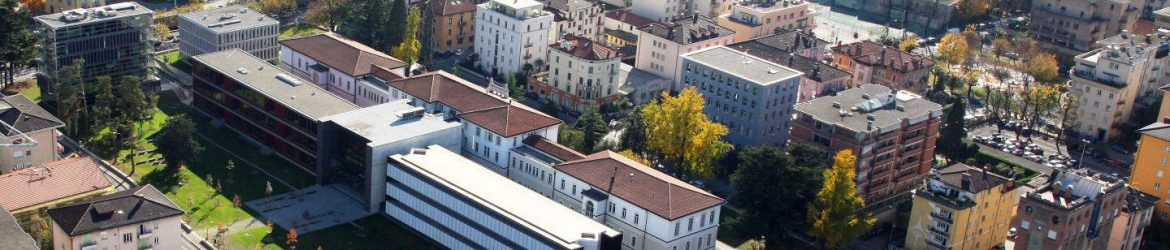
\includegraphics[width=\linewidth]{usi1.jpg}
    \caption{West USI Campus 
        \href{https://uc.inf.usi.ch/wp-content/uploads/2016/07/banner-arial-1170x250.jpg}{(image source)}}
    \label{figure:1}
\end{figure}


USI is the only university in Switzerland where the official language is Italian. It counts
four Faculties at the Lugano campus (Communication Sciences, Economics, Informatics, and
Biomedical Sciences), and the Academy of Architecture at the Mendrisio campus. Affiliated
to USI, since 2010, are the Institute for Research in Biomedicine (IRB) and, from 2017, the
Institute of Oncology Research (IOR), both located in Bellinzona. As of 2021, USI is ranked
251-300 in the THE World University Rankings 2021 \cite{wur}. Table \ref{table:1} shows the distribution of
USI population.

\begin{table}[h]
    \centering
    \caption{USI population stat}
    \begin{tabularx}
    {0.6\textwidth}
    {>{\raggedright\arraybackslash}X >{\raggedleft\arraybackslash}X}
        \hline
        \textbf{Type}           & \textbf{Population}\\
        \hline\hline
        Academic staff          & 869 \\
        Administrative staff    & 190 \\
        Students                & 2,815 \\
        Undergraduates          & 1,342 \\
        Postgraduates           & 1,121 \\
        Doctoral students       & 272 \\
        \hline
        \textbf{Total}          & \textbf{6,609} \\
        \hline
    \end{tabularx}
    \label{table:1}
\end{table}


\newpage
%%%%%%%%%%%%%%%%%%%%%%%%%%%%%%%%%%%%%%%%%%%%%%%%%%%%%%%%%%%%%%%%%%%%%%%%%%%%%%%%%%%%%%%%%%%%%%%
\section{Organization and research areas}
\label{section:2}

\begin{multicols}{2}
USI is active in several studies and research areas: architecture, communication sciences, computational science, data science, economics, health studies, humanities, informatics, law, medicine and biomedicine.
The university is organised in five Departments (Faculties), located on four campuses.
The Faculties of Economics, Communication Sciences, Informatics and Biomedical Sciences are located on two different campuses in Lugano, home also to the Facolt`a di Teologia di Lugano, a private institution affiliated with the Diocese of the Catholic Church in Lugano.
The Accademia di architettura is located on the Mendrisio campus. The affiliated Institute for Research in Biomedicine (IRB) and the Institute of Oncology Research (IOR) are both located in Bellinzona.

\subsection{Architecture}
The Academy of Architecture, founded by acclaimed Swiss architect Mario Botta, is currently headed by Director Walter Angonese.
With forty lecturers and twenty-five design studios (including Mario Botta, Massimo Carmassi, Valerio Olgiati), the Accademia di architettura trains an overall of 764 students for 3-year Bachelor and 2-year master’s degrees (2013).

\subsection{Economics}
The Faculty of Economics is headed by dean Gianluca Colombo.
856 students were registered under the Faculty of Economics (2018).
Main research and teaching topics include: Banking, Finance, Management, Economics and International Policies, Financial Communication, Marketing.

\subsection{Communication sciences}
The Faculty of Communication Sciences is headed by dean Gianluca Colombo.
It is the third largest faculty of USI with 763 students enrolled in the autumn semester 2018-2019.
Topics of research and teaching include Media, new media and journalism, Marketing, Corporate Communication, Public communication, Healthcare communication, Information and communication technologies, Education and Tourism.

\subsection{Informatics}
\label{section:2.4}
The Faculty of Informatics (see Figure \ref{figure:2}) was founded by Mehdi Jazayeri \cite{mj} in 2004. The
current dean is Professor Marc Langheinrich.
\textbf{It is ranked first in Europe for software engineering research, according to CSrankings \cite{cr}}.
The Faculty of Informatics at Universit\`a della Svizzera italiana performs world-class research in many areas of informatics.
With its award-winning, innovative curriculum, the Faculty aims to train informatics experts who are interdisciplinary in approach, with abstract thinking and generalization skills, a sound knowledge in the application fields of information technologies, as well as project management and teamwork abilities.
First year students cover mathematical topics, computer architecture, networking, and fundamental concepts of programming.
A further course persists throughout the 3-year undergraduate curriculum.
Called the Atelier, it has the purpose of bringing the courses together and to provide exposure to real world tools that are useful to computer scientists.
Students are expected to learn about a wide variety of topics, from big O notation and calculus, through networking protocols and layers, to computer architecture.
A variety of programming languages are used.
\end{multicols}
%%%%%%%%%%%%%%%%%%%%%%%%%%%%%%%%%%%%%%%%%%%%%%%%%%%%%%%%%%%%%%%%%%%%%%%%%%%%%%%%%%%%%%%%%%%%%%%
%image
\begin{figure}[t!]
    \centering
    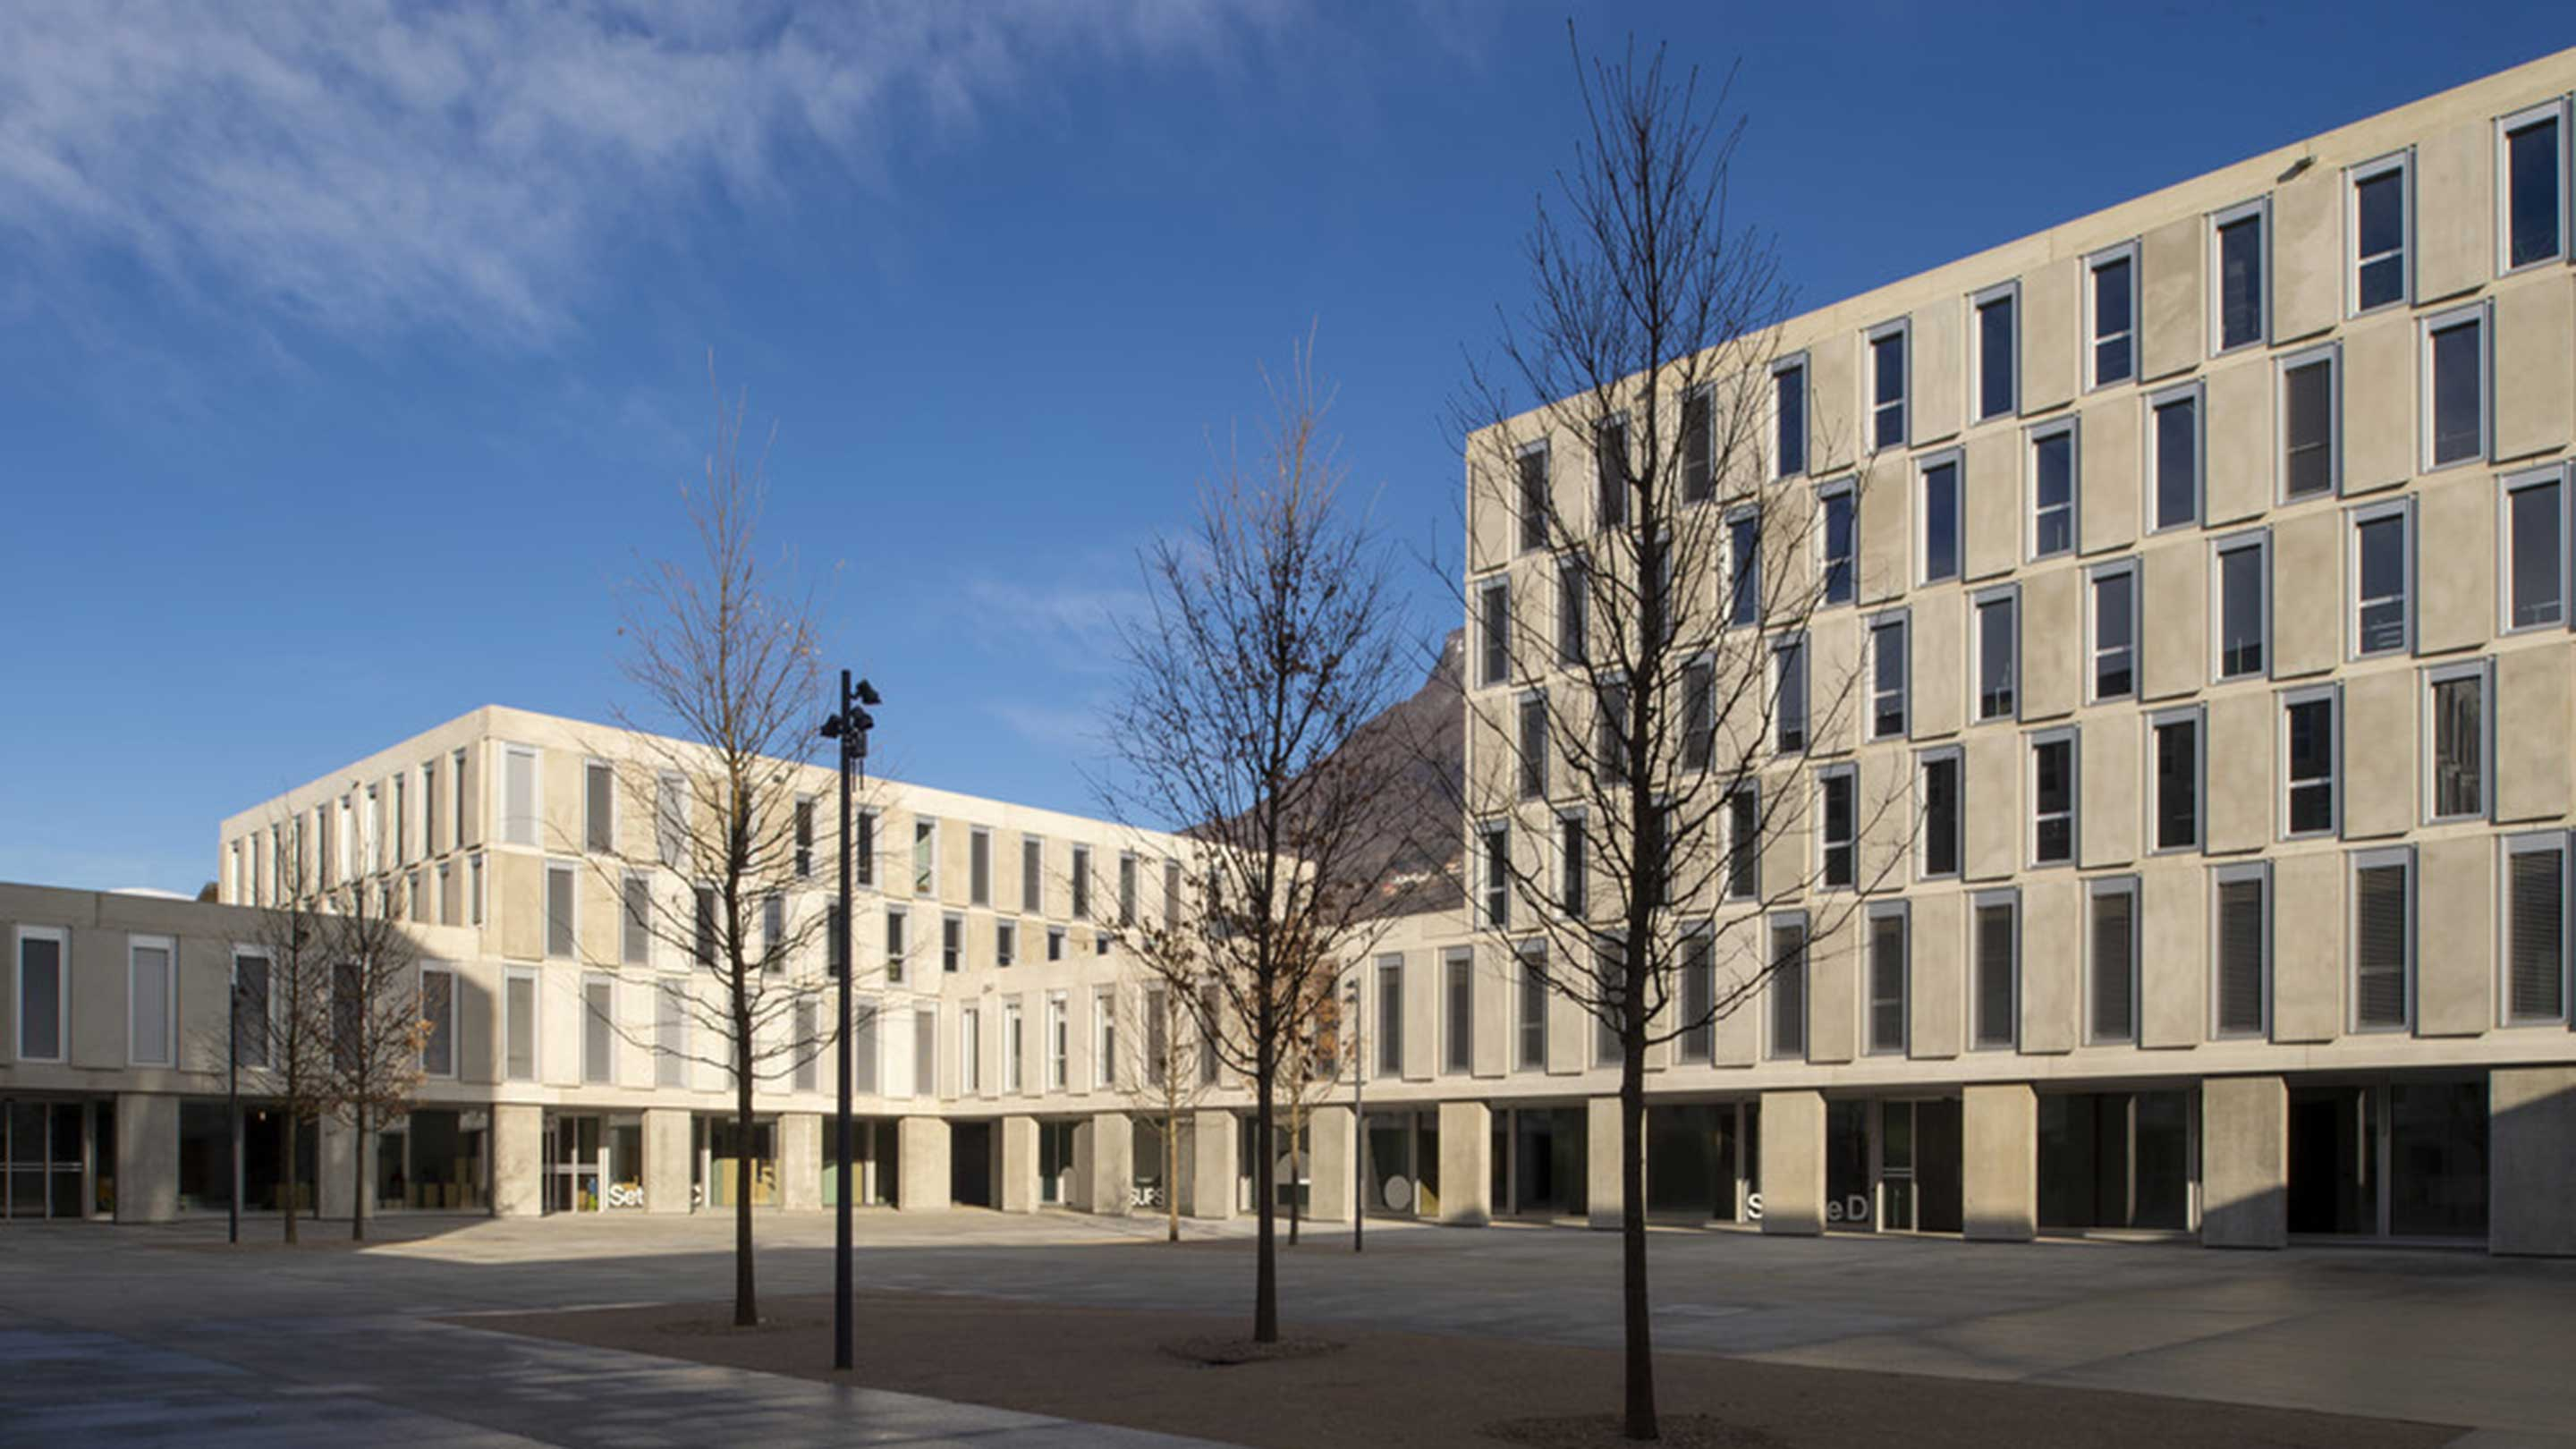
\includegraphics[width=\linewidth]{usi2.jpg}
    \caption{Informatics Building 
        \href{https://www.usi.ch/sites/default/files/storage/images/press-usi-campus-est-01.jpg}{(image source)}}
    \label{figure:2}
\end{figure}

\begin{multicols}{2}
Programming is introduced through Scheme and functional programming throughout the first semester, in parallel with the computer architecture course (which uses MIPS assembly).
Later on, C, Java, and JavaScript are used.
The curriculum puts a strong emphasis on teamwork, with a major group project happening in every semester.\\\\
\textbf{Master topics include:}
\begin{itemize}
  \setlength{\itemsep}{1.2pt}
  \setlength{\parskip}{0.2pt}
  \setlength{\parsep}{0pt}
    \item Software and Data Engineering
    \item Artificial Intelligence
    \item Management and Informatics
    \item Financial Technology and Computing
    \item Informatics
\end{itemize}

\subsection{Biomedical Sciences}
The Faculty of Biomedical Sciences at USI was established in 2014, with the purpose to make a contribution towards the solution of an important problem in Switzerland: the dearth of physicians trained in Switzerland.
The new Faculty offers a master’s degree in Medicine (3-year curriculum), starting in 2020, in close collaboration with ETH Zurich, University of Basel and University of Zurich on the academic side, and with the Ente Ospedaliero Cantonale (EOC) and private clinics in Ticino for bedside teaching.
\end{multicols}
\newpage
%%%%%%%%%%%%%%%%%%%%%%%%%%%%%%%%%%%%%%%%%%%%%%%%%%%%%%%%%%%%%%%%%%%%%%%%%%%%%%%%%%%%%%%%%%%%%%%
\begin{thebibliography}{999}
\bibitem{wur} 
    \href{https://www.timeshighereducation.com/world-university-rankings/2021/world-ranking\#!/page/0/length/25/sort\_by/rank/sort\_order/asc/cols/stats}
    {\textit{“World University Rankings”}}
    Times Higher Education (THE).

\bibitem{mj} 
    \textit{"Mehdi Jazayeri"},
    wikipedia page, 
    \href{https://en.wikipedia.org/wiki/Mehdi_Jazayeri}
        {\textbf{https://en.wikipedia.org/wiki/Mehdi\_Jazayeri}}.

\bibitem{cr} \textit{"CS Ranking"}, 
    \href{https://csrankings.org/#/index?soft&europe}
        {\textbf{https://csrankings.org/\#/index?soft\&europe}}.
\end{thebibliography}

\end{document}
